\documentclass[border=2pt]{standalone}
\usepackage{tikz}
\usetikzlibrary{arrows.meta,positioning}
\begin{document}
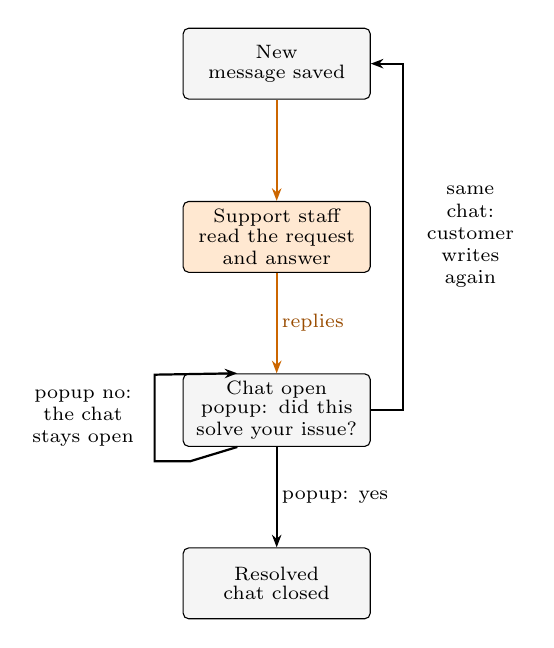
\begin{tikzpicture}[
  every node/.style={font=\scriptsize},
  st/.style={draw, rounded corners=2pt, minimum height=9mm, text width=22mm, align=center, inner sep=2.5pt},
  fx/.style={st, fill=gray!8},
  pr/.style={st, fill=orange!18},
  ar/.style={-{Stealth[length=1.6mm]}, thick},
  ao/.style={ar, draw=orange!80!black},
  lw/.style={font=\scriptsize, inner sep=1.5pt, fill=white},
  lo/.style={lw, text=orange!60!black},
  ls/.style={font=\scriptsize, inner sep=1.5pt, fill=white, text width=13mm, align=center}]
  \node[fx] (new) at (0,0) {New\\[-1pt]{\scriptsize message saved}};
  \node[pr] (sta) at (0,-2.2) {Support staff\\[-1pt]{\scriptsize read the request and answer}};
  \node[fx] (cha) at (0,-4.4) {Chat open\\[-1pt]{\scriptsize popup: did this solve your issue?}};
  \node[fx] (res) at (0,-6.6) {Resolved\\[-1pt]{\scriptsize chat closed}};

  \draw[ao] (new) -- (sta);
  \draw[ao] (sta) -- node[lo, right]{replies} (cha);
  \draw[ar] (cha) -- node[lw, right]{popup: yes} (res);
  \draw[ar] (cha.east) -- (1.6,-4.4) -- (1.6,0) -- (new.east);
  \node[ls, right] at (1.75,-2.2) {same chat: customer writes again};
  \draw[ar] ([xshift=-5mm]cha.south) -- (-1.1,-5.05) -- (-1.55,-5.05) -- (-1.55,-3.95) -- ([xshift=-5mm]cha.north);
  \node[ls, left] at (-1.75,-4.5) {popup no: the chat stays open};
\end{tikzpicture}
\end{document}
